\chapter{Implementation}
\label{cha:implementation}
In this chapter, we describe how we implemented the simulation. First, section~\ref{sec:components} presents the various components we developed by describing what their task is, what we noticed during the implementation and why we implemented it this way. \textcolor{red}{module dependencies extra or in modules?} In section~\ref{sec:module_dependencies}, we describe the dependencies and interaction between the modules we developed. Section~\ref{sec:imp_communication} covers the implementation of the communication between Fawkes and Gazebo and between multiple robots we want to simulate. In section~\ref{sec:agent_improvements}, we present the improvements for the multi-agent system we implemented during the thesis.

\section{Components}
\label{sec:components}
\subsection{Gazebo Models}
\begin{figure}
\centering
\begin{subfigure}[b]{0.48\textwidth}
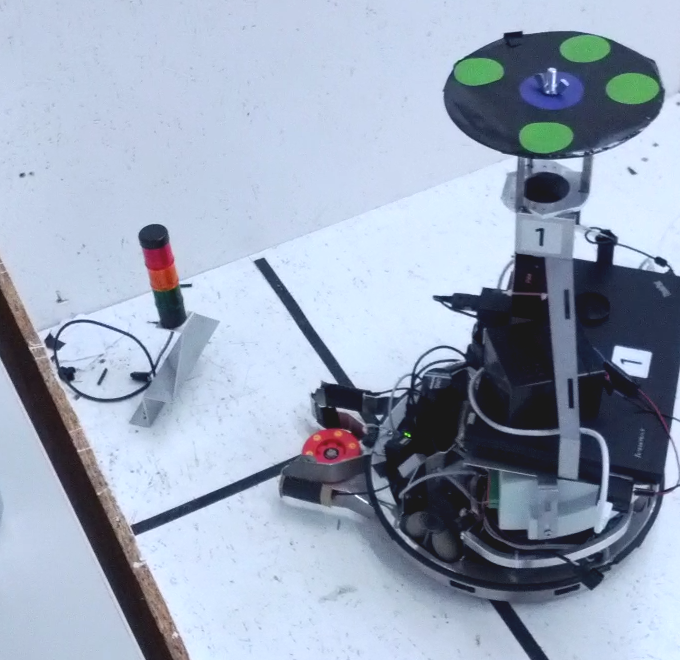
\includegraphics[width=\textwidth]{pics/llsf_real}
\caption{A Robotino delivers a puck to a recycling machine.}
\label{fig:comparison_real}
\end{subfigure}
\begin{subfigure}[b]{0.48\textwidth}
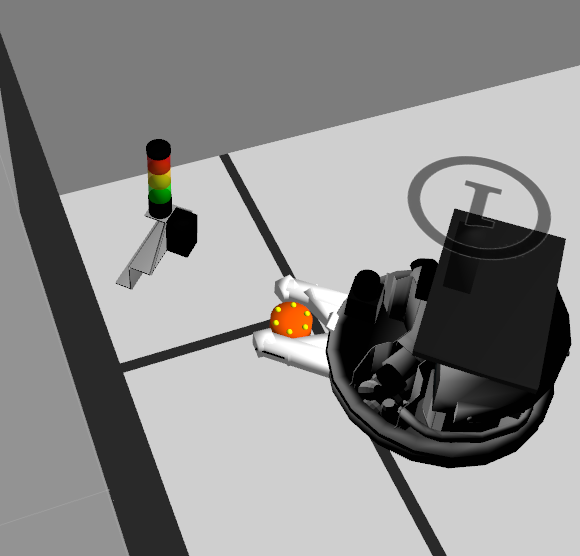
\includegraphics[width=\textwidth]{pics/llsf_sim}
\caption{The same situation in the Gazebo~simulation}
\label{fig:comparison_sim}
\end{subfigure}
\caption{Comparison of the real scene and the simulated scene in Gazebo}
\label{fig:comparison}
\end{figure}

In order to simulate the LLSF environment, we need to model all objects appearing in this domain. Here, we present our simulation models and why we modeled them this way. Figure~\ref{fig:comparison} shows a comparison between a real LLSF scene and the same scene in the simulation. In this comparison, the most important objetcs of the simulation can be seen. In the following we descibe each model in detail:\\
\textbf{LLSF Field:} The model of the LLSF field has a rather simple structure. It consists of a ground plate and four side walls. For the visual apperance and possible future changes, the field has a visual representation with lines and colored areas just as on the real field. The machines are not realized as a component of the field and are attached to the field in the description of the simulation world.\\
\textbf{Mashine:} The model of the machines matches the real machines structurally. Though, it is challenging to represent the lamps consisting of colored plexiglass and a LED \textcolor{red}{abbreviation?} inside. We decided to use simple colored cylinders in the simulation. If the lamp is turned off, we use a dark and slightly transparent color and, if the light is turned on, we use a a bright color. This looks reasonable in the simulation and the images from the simulation are sufficient for our vision plugin which determines the lamp state of the machines. The vision plugin measures the brightness at the position where it expects the machine-lamp to be and it even was not necessary to change brightness thresholds. In Figure~\ref{fig:comparison_real}, the black RFID box in front of the machine is missing because we currently do not have the RFID readers.\\
\textbf{Puck:} The visual appearence of the puck model can be seen in Figure~\ref{fig:comparison_sim}. Physically, they are represented by a single cylinder. The difficult part was to find good friction parameters for the surface of the cylinder. On the one hand, it should be easy to slide the puck across the floor. On the other hand, the puck should stay inside the gripper of the Robotino when the Robotino turns. If the friction parameters are too small, the pucks move outside the gripper while turning because of the centrifugal force. \textcolor{red}{mention other solution?}\\
\textbf{Robotiono:} The model of the robotino is the most complex model because it holds different sensors, the casing and the puck gripper. It is also the most important one because it represents the robot we want to simulate. The major visual difference between real world and simulation is caused by the missing framework on top of the Robotino and the visual apperance of the puck gripper. Both is not important because we do net detect other Robotinos with a camera. We detect them with the laser sensor. Therefore and because of the manipulation with the gripper, the physical representation is more important. \textcolor{red}{collisions picture?} The physical model of the Robotino is composed of the gripper and two cylinders, one on the ground to represent the basic circle of the Robotino and one on laser and machine height. The cylinder on laser height is smaller and shifted back so that it does not block the laser sensor of the same Robotino and it fits better to the real shape. The gripper in the simulation has a similar shape than the real one. We needed to assign higher friction parameters to the inside of the gripper than to the outside because in reality the puck slides into the gripper if the front side of the gripper and stays in the gripper while turning. Because we were not able to simulate this with a single set of friction parameters, we modeled an additional geometry for the inside of the gripper with higher friction parameters. Originally, we intended to add wheels to the physical design for the final version. However, the omni-directional wheels caused an abnormal physical behavior in the simulation. The wheels irregularly bounced on the ground because of gravity and collision. Because we could not solve this problem in an arguable time and there is no important advange, we decided to stay at the simple model without wheels. We only loose the posibility to physically simulate the odometry with its error. Therefore we introduced an artificially odometry error in the Gazebo plugin for the Robotino. \textcolor{red}{friction, setvel?}\\
\textbf{Simulation World:} The world file combines the developed models to an LLSF environment. Our world consists of the LLSF field, 16 machines with configurable orientation, 20 pucks and three Robotinos.\\


\subsection{Gazebo Plugins}
\textbf{World Plugin}
\\
\textbf{Robotino Plugin}


\subsection{Fawkes Plugins}
\subsection{Automation Scripts}


\section{Module Dependencies}
\label{sec:module_dependencies}


\section{Communication}
\label{sec:imp_communication}


\section{Agent Improvements}
\label{sec:agent_improvements}
dynamic role switch: no more products ordered, \cite{dynamic_role_assignment}
